\documentclass[a4paper,12pt]{article}

\usepackage[T2A]{fontenc}			
\usepackage[utf8]{inputenc}			
\usepackage[english,russian]{babel}	

\usepackage[
bookmarks=true, colorlinks=true, unicode=true,
urlcolor=black,linkcolor=black, anchorcolor=black,
citecolor=black, menucolor=black, filecolor=black,
]{hyperref}

\usepackage{color}
\usepackage{caption}
\DeclareCaptionFont{white}{\color{black}}
\DeclareCaptionFormat{listing}{\colorbox{white}{\parbox{\textwidth}{#1#2#3}}}

\usepackage{amsmath,amsfonts,amssymb,amsthm,mathtools} 
\usepackage{wasysym}

\usepackage[cache=false]{minted}

\usepackage{graphicx}
\usepackage{cmap}
\usepackage{indentfirst}

\usepackage{listings} 
\usepackage{fancyvrb}

\usepackage{geometry}
\geometry{left=2cm}
\geometry{right=1.5cm}
\geometry{top=1cm}
\geometry{bottom=2cm}

\usepackage{longtable}

\setlength{\parindent}{5ex}
\setlength{\parskip}{0.5em}

\usepackage{pgfplots}
\usetikzlibrary{datavisualization}
\usetikzlibrary{datavisualization.formats.functions}

\begin{document}
	\lstset{ %
		language=C,                 % выбор языка для подсветки (здесь это С)
		basicstyle=\small\sffamily, % размер и начертание шрифта для подсветки кода
		numbers=left,               % где поставить нумерацию строк (слева\справа)
		numberstyle=\tiny,           % размер шрифта для номеров строк
		stepnumber=1,                   % размер шага между двумя номерами строк
		numbersep=5pt,                % как далеко отстоят номера строк от подсвечиваемого кода
		backgroundcolor=\color{white}, % цвет фона подсветки - используем \usepackage{color}
		showspaces=false,            % показывать или нет пробелы специальными отступами
		showstringspaces=false,      % показывать или нет пробелы в строках
		showtabs=false,             % показывать или нет табуляцию в строках
		frame=single,              % рисовать рамку вокруг кода
		tabsize=2,                 % размер табуляции по умолчанию равен 2 пробелам
		captionpos=t,              % позиция заголовка вверху [t] или внизу [b] 
		breaklines=true,           % автоматически переносить строки (да\нет)
		breakatwhitespace=false, % переносить строки только если есть пробел
		escapeinside={\%*}{*)}   % если нужно добавить комментарии в коде
	}

	% Титульный лист
	\begin{figure}[h!]
		\begin{center}
			{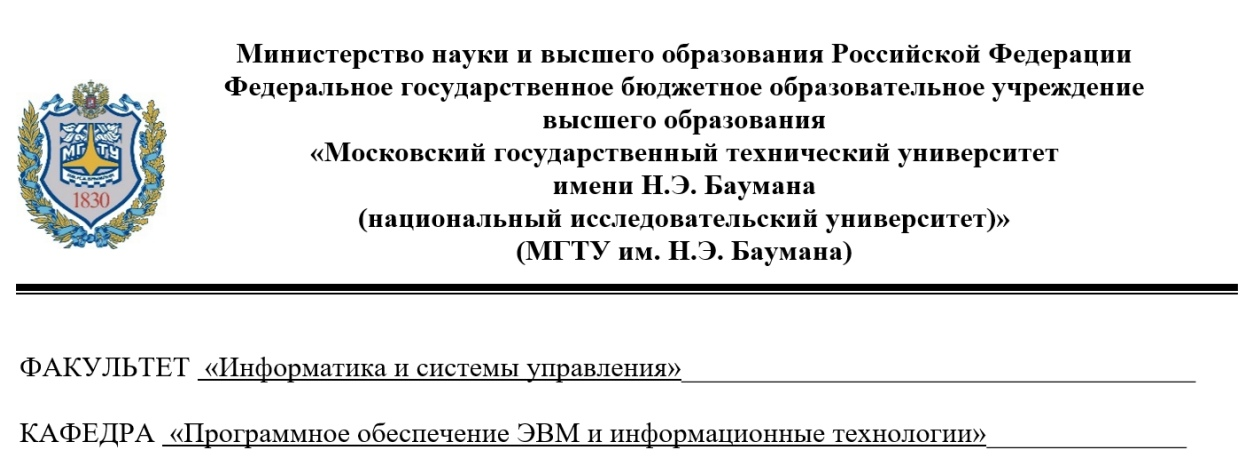
\includegraphics[scale = 0.4]{titul.jpg}}
			\label{titul}
		\end{center}
	\end{figure}
	
	\vspace*{15mm} 
	
	\huge
	\begin{center}
		Дисциплина: <<Функциональное и логическое программирование>>
	\end{center}
	\vspace*{15mm} 	
	
	\begin{center}
		Исправление ошибок 14, 15, 16 лабораторных работ
	\end{center}
	
	\vspace*{15mm} 	
	
	\large
	\begin{flushright}
		Студент: Левушкин И. К. \\
		Группа: ИУ7-62Б \\
		Преподаватели: Толпинская Н. Б., \\ Строганов Ю. В. \\
	\end{flushright}
	
	\vspace*{30mm}
	\begin{center}
		Москва, 2020 г.  
	\end{center}
	\thispagestyle{empty}
	
	
	\newpage

	\section*{Исправление ошибок 15-ой лабораторной работы}
	
	\subsection*{Замечание}
	
	\textit{В таблице странная нотация: != в Prolog символ ! – значимый}
	
	\textit{Подстановка Building = moscow\_city, Building\_Cost =
		987654321. Это множество – нотация: \{…\}
}
	
	\subsubsection*{Исправленная таблица для поиска <<Названия и стоимости всех объектов собственности по заданному субъекту>>}
	
	\textit{Порядок работы системы на 3 примере:}
	
	\begin{minted}{prolog}
	goal
	owner(ryazanova, area_owner(Area, Area_Cost));
	owner(ryazanova, building_owner(Building, Building_Cost));
	owner(ryazanova, watercraft_owner(Watercraft, Watercraft_Cost));
	owner(ryazanova, car_owner(Car, _, Car_Cost, _)).
	%Вывод:
	Building=moscow_city, Building_Cost=987654321
	Car=bugatti, Car_Cost=999999999
	2 Solutions
	\end{minted}
	
	\begin{center}
		\begin{longtable}[h!]{|p{0.05\linewidth}|p{0.5\linewidth}|p{ 0.4\linewidth}|}
			\hline
			{\bf  № шага} & {\bf Сравниваемые термы; результат; 
				
				подстановка, если есть} & {\bf Дальнейшие действия: прямой ход 
				
				или откат (к чему приводит?)} \\
			\hline
			{1} & {T1 = owner(ryazanova, area\_owner(Area, Area\_Cost));
				
				T2 = get\_own\_cost(Sername, building, Cost).
				
				Неудача (функторы owner и get\_own\_cost не равны).} & {Прямой ход к следующему предложению. Аналогичная ситуация в следующих 5 предложениях. Прямой ход к следующему предложению}\\
			\hline
			{7} & {T1 = owner(ryazanova, area\_owner(Area, Area\_Cost));
				
				T2 = owner(Sername, car\_owner(Model, Color, Cost, Probeg)).
				
				Неудача (функторы area\_owner и car\_owner не равны).} & {Прямой ход к следующему предложению.}\\
			\hline
			{8} & {T1 = owner(ryazanova, area\_owner(Area, Area\_Cost));
				
				T2 = owner(levushkin, building\_owner(dacha, 90000)).
				
				Неудача (ryazanova не равно levushkin).} & {Прямой ход к следующему предложению.}\\
			\hline
			{9} & {T1 = owner(ryazanova, area\_owner(Area, Area\_Cost));
				
				T2 =  owner(levushkin, area\_owner(dacha\_area, 9000).
				
				Неудача (ryazanova не равно levushkin)} & {Прямой ход к следующему предложению.}\\
			\hline
			{10} & {T1 = owner(ryazanova, area\_owner(Area, Area\_Cost));
				
				T2 =  owner(levushkin, warercraft\_owner(boat, 90)).
				
				Неудача (ryazanova не равно levushkin)} & {Прямой ход к следующему предложению.}\\
			\hline
			{11} & {T1 = owner(ryazanova, area\_owner(Area, Area\_Cost));
				
				T2 =  owner(samkov, building\_owner(fitness\_club, 888888)).
				
				Неудача (ryazanova не равно samkov).} & {Прямой ход к следующему предложению.}\\
			\hline
			{12} & {T1 = owner(ryazanova, area\_owner(Area, Area\_Cost));
				
				T2 =  owner(samkov, area\_owner(park, 89898989)).
				
				Неудача (ryazanova не равно samkov).} & {Прямой ход к следующему предложению.}\\
			\hline
			{13} & {T1 = owner(ryazanova, area\_owner(Area, Area\_Cost));
				
				T2 =  owner(ryazanova, building\_owner(moscow\_city, 987654321)).
				
				Неудача (функторы area\_owner и building\_owner не равны).} & {Прямой ход к следующему предложению.}\\
			\hline
			{14} & {T1 = owner(ryazanova, area\_owner(Area, Area\_Cost));
				
				T2 =  phone\_list(levushkin, <<89859771492>>, adr(moscow, kantemirovskaya, 5, 1)).
				
				Неудача (функторы owner и phone\_list не равны).} & {Прямой ход к следующему предложению. Аналогичная ситуация в следующих 9 предложениях (phone\_list, auto, bank\_list). Откат, переход к предыдущему состоянию резольвенты. Поиск с начала предложений.}\\
			\hline
			{24} & {T1 = owner(ryazanova, building\_owner(Building, Building\_Cost));
				
				T2 = get\_own\_cost(Sername, building, Cost).
				
				Неудача (функторы owner и get\_own\_cost не равны).} & {Прямой ход к следующему предложению. Аналогичная ситуация в следующих 5 предложениях. Прямой ход к следующему предложению}\\
			\hline
			{30} & {T1 = owner(ryazanova, building\_owner(Building, Building\_Cost));
				
				T2 = owner(Sername, car\_owner(Model, Color, Cost, Probeg)).
				
				Неудача (функторы building\_owner и car\_owner не равны).} & {Прямой ход к следующему предложению.}\\
			\hline
			{31} & {T1 = owner(ryazanova, building\_owner(Building, Building\_Cost));
				
				T2 = owner(levushkin, building\_owner(dacha, 90000)).
				
				Неудача (ryazanova не равно levushkin).} & {Прямой ход к следующему предложению.}\\
			\hline
			{32} & {T1 = owner(ryazanova, building\_owner(Building, Building\_Cost));
				
				T2 =  owner(levushkin, area\_owner(dacha\_area, 9000).
				
				Неудача (ryazanova не равно levushkin)} & {Прямой ход к следующему предложению.}\\
			\hline
			{33} & {T1 = owner(ryazanova, building\_owner(Building, Building\_Cost));
				
				T2 =  owner(levushkin, warercraft\_owner(boat, 90)).
				
				Неудача (ryazanova не равно levushkin)} & {Прямой ход к следующему предложению.}\\
			\hline
			{34} & {T1 = owner(ryazanova, building\_owner(Building, Building\_Cost));
				
				T2 =  owner(samkov, building\_owner(fitness\_club, 888888)).
				
				Неудача (ryazanova не равно samkov).} & {Прямой ход к следующему предложению.}\\
			\hline
			{35} & {T1 = owner(ryazanova, building\_owner(Building, Building\_Cost));
				
				T2 =  owner(samkov, area\_owner(park, 89898989)).
				
				Неудача (ryazanova не равно samkov).} & {Прямой ход к следующему предложению.}\\
			\hline
			{36} & {T1 = owner(ryazanova, building\_owner(Building, Building\_Cost));
				
				T2 =  owner(ryazanova, building\_owner(moscow\_city, 987654321)).
				
				Успех. Подсановка \{Building = moscow\_city, Building\_Cost = 987654321\}.} & {Вывод:
				
				Building = moscow\_city,
				
				Building\_Cost = 987654321,
				
				Прямой ход к следующему предложению. Реконкретизация Building, Building\_Cost.}\\
			\hline
			{37} & {T1 = owner(ryazanova, building\_owner(Building, Building\_Cost));
				
				T2 =  phone\_list(levushkin, <<89859771492>>, adr(moscow, kantemirovskaya, 5, 1)).
				
				Неудача (функторы owner и phone\_list не равны).} & {Прямой ход к следующему предложению. Аналогичная ситуация в следующих 9 предложениях (phone\_list, auto, bank\_list). Откат, переход к предыдущему состоянию резольвенты. Поиск с начала предложений.}\\
			\hline
			{47} & {T1 = owner(ryazanova, watercraft\_owner(Watercraft, Watercraft\_Cost));
				
				T2 = get\_own\_cost(Sername, building, Cost).
				
				Неудача (функторы owner и get\_own\_cost не равны).} & {Прямой ход к следующему предложению. Аналогичная ситуация в следующих 5 предложениях. Прямой ход к следующему предложению}\\
			\hline
			{53} & {T1 = owner(ryazanova, watercraft\_owner(Watercraft, Watercraft\_Cost));
				
				T2 = owner(Sername, car\_owner(Model, Color, Cost, Probeg)).
				
				Неудача (функторы watercraft\_owner и car\_owner не равны).} & {Прямой ход к следующему предложению.}\\
			\hline
			{54} & {T1 = owner(ryazanova, watercraft\_owner(Watercraft, Watercraft\_Cost));
				
				T2 = owner(levushkin, building\_owner(dacha, 90000)).
				
				Неудача (ryazanova не равно levushkin).} & {Прямой ход к следующему предложению.}\\
			\hline
			{55} & {T1 = owner(ryazanova, watercraft\_owner(Watercraft, Watercraft\_Cost));
				
				T2 =  owner(levushkin, area\_owner(dacha\_area, 9000).
				
				Неудача (ryazanova не равно levushkin)} & {Прямой ход к следующему предложению.}\\
			\hline
			{56} & {T1 = owner(ryazanova, watercraft\_owner(Watercraft, Watercraft\_Cost));
				
				T2 =  owner(levushkin, warercraft\_owner(boat, 90)).
				
				Неудача (ryazanova не равно levushkin)} & {Прямой ход к следующему предложению.}\\
			\hline
			{57} & {T1 = owner(ryazanova, watercraft\_owner(Watercraft, Watercraft\_Cost));
				
				T2 =  owner(samkov, building\_owner(fitness\_club, 888888)).
				
				Неудача (ryazanova не равно samkov).} & {Прямой ход к следующему предложению.}\\
			\hline
			{58} & {T1 = owner(ryazanova, watercraft\_owner(Watercraft, Watercraft\_Cost));
				
				T2 =  owner(samkov, area\_owner(park, 89898989)).
				
				Неудача (ryazanova не равно samkov).} & {Прямой ход к следующему предложению.}\\
			\hline
			{59} & {T1 = owner(ryazanova, watercraft\_owner(Watercraft, Watercraft\_Cost));
				
				T2 =  owner(ryazanova, building\_owner(moscow\_city, 987654321)).
				
				Неудача (функторы watercraft\_owner и building\_owner не равны).} & {Прямой ход к следующему предложению.}\\
			\hline
			{60} & {T1 = owner(ryazanova, watercraft\_owner(Watercraft, Watercraft\_Cost));
				
				T2 =  phone\_list(levushkin, <<89859771492>>, adr(moscow, kantemirovskaya, 5, 1)).
				
				Неудача (функторы owner и phone\_list не равны).} & {Прямой ход к следующему предложению. Аналогичная ситуация в следующих 9 предложениях (phone\_list, auto, bank\_list). Откат, переход к предыдущему состоянию резольвенты. Поиск с начала предложений.}\\
			\hline
			{70} & {T1 = owner(ryazanova, car\_owner(Car, \_, Car\_Cost, \_));
				
				T2 = get\_own\_cost(Sername, building, Cost).
				
				Неудача (функторы owner и get\_own\_cost не равны).} & {Прямой ход к следующему предложению. Аналогичная ситуация в следующих 5 предложениях. Прямой ход к следующему предложению}\\
			\hline
			{76} & {T1 = owner(ryazanova, car\_owner(Car, \_, Car\_Cost, \_));
				
				T2 = owner(Sername, car\_owner(Model, Color, Cost, Probeg)).
				
				Успех. Подстановка \{ryazanova = Sername, Car = Model, Car\_Cost = Cost\}.} & {Прямой ход к auto(ryazanova, Car, \_, Car\_Cost, \_). Поиск с начала предложений.}\\
			\hline
			{77} & {T1 = auto(ryazanova, Car, \_, Car\_Cost, \_);
				
				T2 = get\_own\_cost(Sername, building, Cost).
				
				Неудача (функторы auto и get\_own\_cost не равны).} & {Прямой ход к следующему предложению. Аналогичная ситуация в следующих 15 предложениях (get\_own\_cost, get\_sum\_cost\_owner, owner, phone\_list). Прямой ход к следующему предложению}\\
			\hline
			{93} & {T1 = auto(ryazanova, Car, \_, Car\_Cost, \_);
				
				T2 = auto(levushkin, volvo, grey, 3000000, 1000).
				
				Неудача (ryazanova не равно levushkin).} & {Прямой ход к следующему предложению.}\\
			\hline
			{94} & {T1 = auto(ryazanova, Car, \_, Car\_Cost, \_);
				
				T2 = auto(samkov, volkswagen, pink, 1000000, 99999).
				
				Неудача (ryazanova не равно samkov).} & {Прямой ход к следующему предложению.}\\
			\hline
			{95} & {T1 = auto(ryazanova, Car, \_, Car\_Cost, \_);
				
				T2 = auto(ryazanova, bugatti, gold, 999999999, 1).
				
				Успех. Подстановка \{Car = bugatti, Car\_Cost = 999999999\}.} & {Вывод: Car = bugatti, Car\_Cost = 999999999. Прямой ход к следующему предложению, реконкретизация Car, Car\_Cost.}\\
			\hline
			{96} & {T1 = auto(ryazanova, Car, \_, Car\_Cost, \_);
				
				T2 = bank\_list(levushkin, sberbank, 1111, 900000).
				
				Неудача (функторы auto и bank\_list не равны).} & {Прямой ход к следующему предложению. Аналогичная ситуация в следующих 3 предложениях. Откат, переход к предыдущему состоянию резольвенты - owner(ryazanova, car\_owner(Car, \_, Car\_Cost, \_)), реконкретизация Car, Car\_Cost.}\\
			\hline
			{100} & {T1 = owner(ryazanova, car\_owner(Car, \_, Car\_Cost, \_));
				
				T2 = owner(levushkin, building\_owner(dacha, 90000).
				
				Неудача (ryazanova не равно levushkin).)} & {Прямой ход к следующему предложению. Аналогичная ситуация в следующих 2 предложениях. Прямой ход к следующему предложению.}\\
			\hline
			{103} & {T1 = owner(ryazanova, car\_owner(Car, \_, Car\_Cost, \_));
				
				T2 = owner(samkov, building\_owner(fitness\_club, 888888)).
				
				Неудача (ryazanova не равно samkov).} & {Прямой ход к следующему предложению. Аналогичная ситуация в следующем предложении. Прямой ход к следующему предложению.}\\
			\hline
			{105} & {T1 = owner(ryazanova, car\_owner(Car, \_, Car\_Cost, \_));
				
				T2 = owner(ryazanova, building\_owner(moscow\_city, 987654321)).
				
				Неудача (функторы car\_owner и building\_owner не равны).} & {Прямой ход к следующему предложению.}\\
			\hline
			{106} & {T1 = owner(ryazanova, car\_owner(Car, \_, Car\_Cost, \_));
				
				T2 = phone\_list(levushkin, <<89859771492>>, adr(moscow, kantemirovskaya, 5, 1)).
				
				Неудача (функторы owner и phone\_list не равны).} & {Прямой ход к следующему предложению. Аналогичная ситуация в следующих 9 предложениях (phone\_list, auto, bank\_list). Откат, переход к предыдущему состоянию резольвенты. Конец clauses. Опустошение резольвенты. Завершение работы (115 шагов).}\\
			\hline
			\label{m1}
		\end{longtable}
	\end{center}
	
	
	\subsection*{Замечание}
	
	\textit{Правило:}
	
	\textit{get\_sum\_cost\_owner(Sername, Cost) :- }
	
	\textit{get\_own\_cost(Sername, building, Building\_Cost),}
	
	\textit{get\_own\_cost(Sername, area, Area\_Cost),}
	
	\textit{get\_own\_cost(Sername, watercraft, Watercraft\_Cost),}
	
	\textit{get\_own\_cost(Sername, car, Car\_Cost),}
	
	\textit{Cost = Building\_Cost + Area\_Cost + Watercraft\_Cost + Car\_Cost.}
	
	\textit{ИТЕРАЦИОННЫЙ способ мышления! Эффективнее было бы использовать один, универсальный предикат – <<собственность>>}
	
	\subsubsection*{Исправленный текст программы}
	
	\begin{minted}{prolog}
domains
	town, street, sername, model, 
	watercraft, color, bank, area, building = symbol
	phone = string
	house, case, cost, probeg, account, money = integer
	address = adr(town, street, house, case)
	ownership = building_owner(building, cost) ;area_owner(area, cost)
	 ;watercraft_owner(watercraft, cost)
	 ;car_owner(model, color, cost, probeg)
predicates
	phone_list(sername, phone, address).
	auto(sername, model, color, cost, probeg).
	bank_list(sername, bank, account, money).
	
	owner(sername, ownership).
	
	get_own_cost(sername, ownership, cost, cost).
	
	
	get_sum_cost_owner(sername, cost).
clauses

	get_own_cost(Sername, building_owner(_, _), Cost, Result) :-
	owner(Sername, building_owner(_, Building_Cost)),
	New_cost = Cost + Building_Cost,
	get_own_cost(Sername, area_owner(_, _), New_cost, Result),
	!.
	
	get_own_cost(Sername, building_owner(_, _), Cost, Result):-
	get_own_cost(Sername, area_owner(_, _), Cost, Result),
	!.
	
	get_own_cost(Sername, area_owner(_, _), Cost, Result) :-
	owner(Sername, area_owner(_, Area_Cost)),
	New_cost = Cost + Area_Cost,
	get_own_cost(Sername, watercraft_owner(_, _), New_cost, Result),
	!.
	
	get_own_cost(Sername, area_owner(_, _), Cost, Result):-
	get_own_cost(Sername, watercraft_owner(_, _), Cost, Result),
	!.
	
	get_own_cost(Sername, watercraft_owner(_, _), Cost, Result) :-
	owner(Sername, watercraft_owner(_, Watercraft_Cost)),
	New_cost = Cost + Watercraft_Cost,
	get_own_cost(Sername, car_owner(_, _, _, _), New_cost, Result),
	!.
	
	get_own_cost(Sername, watercraft_owner(_, _), Cost, Result):-
	get_own_cost(Sername, car_owner(_, _, _, _), Cost, Result),
	!.
	
	get_own_cost(Sername, car_owner(_, _, _, _), Cost, Result) :-
	owner(Sername, car_owner(_, _, Car_Cost, _)),
	Result = Cost + Car_Cost,
	!.
	
	get_own_cost(_, car_owner(_, _, _, _), Cost, Cost):-
	!.
	
	
	get_sum_cost_owner(Sername, Cost) :-
	get_own_cost(Sername, building_owner(_, _), 0, Cost).
	
	
	
	owner(Sername, car_owner(Model, Color, Cost, Probeg)) :-
	auto(Sername, Model, Color, Cost, Probeg).
	
	
	owner(levushkin, building_owner(dacha, 90000)).
	owner(levushkin, area_owner(dacha_area, 9000)).
	owner(levushkin, watercraft_owner(boat, 90)).
	
	owner(samkov, building_owner(fitness_club, 888888)).
	owner(samkov, area_owner(park, 89898989)).
	
	owner(ryazanova, building_owner(moscow_city, 987654321)).
	
	
	phone_list(levushkin, "89859771492", 
	adr(moscow, kantemirovskaya, 5, 1)).
	phone_list(samkov, "89899999", 
	adr(chelyabinsk, pushkinskaya, 4, 2)).
	phone_list(ryazanova, "8911911911", 
	adr(moscow, baumanskaya, 9, 9)).
	
	
	auto(levushkin, volvo, grey, 3000000, 1000).
	auto(samkov, volkswagen, pink, 1000000, 99999).
	auto(ryazanova, bugatti, gold, 999999999, 1).
	
	
	bank_list(levushkin, sberbank, 1111, 900000).
	bank_list(samkov, sberbank, 2222, 100).
	bank_list(ryazanova, tinkoff, 3333, 99999999).
	bank_list(ryazanova, raiffeisen, 4444, 888888888).
goal
	%Названия всех объектов собственности по заданному субъекту
	%Пример 1
	owner(levushkin, area_owner(Area, _));
	owner(levushkin, building_owner(Building, _));
	owner(levushkin, watercraft_owner(Watercraft, _));
	owner(levushkin, car_owner(Car, _, _, _)).
	%Пример 2
	owner(samkov, area_owner(Area, _));
	owner(samkov, building_owner(Building, _));
	owner(samkov, watercraft_owner(Watercraft, _));
	owner(samkov, car_owner(Car, _, _, _)).
	%Пример 3
	owner(ryazanova, area_owner(Area, _));
	owner(ryazanova, building_owner(Building, _));
	owner(ryazanova, watercraft_owner(Watercraft, _));
	owner(ryazanova, car_owner(Car, _, _, _)).
	%Названия и стоимости всех объектов собственности 
	%по заданному субъекту
	%Пример 1
	owner(levushkin, area_owner(Area, Area_Cost));
	owner(levushkin, building_owner(Building, Building_Cost));
	owner(levushkin, watercraft_owner(Watercraft, Watercraft_Cost));
	owner(levushkin, car_owner(Car, _, Car_Cost, _)).
	%Пример 2
	owner(samkov, area_owner(Area, Area_Cost));
	owner(samkov, building_owner(Building, Building_Cost));
	owner(samkov, watercraft_owner(Watercraft, Watercraft_Cost));
	owner(samkov, car_owner(Car, _, Car_Cost, _)).
	%Пример 3
	owner(ryazanova, area_owner(Area, Area_Cost));
	owner(ryazanova, building_owner(Building, Building_Cost));
	owner(ryazanova, watercraft_owner(Watercraft, Watercraft_Cost));
	owner(ryazanova, car_owner(Car, _, Car_Cost, _)).
	\end{minted}
	
	\subsection*{Замечание}
	
	\textit{Знания размещены в CLAUSES в виде предложений.}
	\textit{Они представляют собой знания о некоторой предметной области,} \textit{формально – отношения между различными объектами. Не четко!}
	
	\subsubsection*{Исправление}
	
	\textit{Вопрос:} 
	
	В каком фрагменте программы сформулировано знание? Это знание о чем на формальном уровне?

	\textit{Ответ:}
	
	Знания размещены в CLAUSES в виде предложений.
	
	Они представляют собой знания о некоторой предметной области, формально – утверждения : факты и правила.
	
	\subsection*{Замечание}
	
	\textit{С помощью описанных предикатов, можно создавать предложения в базе знаний.}
	
	\textit{Предикаты используются для представления, как фактов, так и правил. Звучит неверн}
	
	\subsubsection*{Исправление}
	
	\textit{Вопрос:}
	
	Какова семантика (смысл) предложений раздела PREDICATES? Когда, и где используется это описание? С какой целью?
	
	\textit{Ответ:}
	
	В разделе PREDICATES описываются предикаты, их арность (местность) и домены (типы и природа аргументов).
	
	С помощью описанных предикатов, описываются процедуры в разделе CLAUSES.
	
	Процедурой называется совокупность правил, заголовки которых имеют одно и то же имя и одну и ту же арность (местность), т.е. это совокупность правил, описывающих одно определенное отношение. 

	\section*{Исправление ошибок 16-ой лабораторной работы}
	
	\subsection*{Замечание}
	
	\textit{tatiana = tatiana  константы в подстановку не заносятся!}
		
	\subsubsection*{Исправленная таблица для вопроса: <<По имени субъекта определить его бабушку и дедушку по материнской линии (предки 2-го колена)>>}
	
	\textit{Текст программы:}
	
	\begin{minted}{prolog}
predicates
	first_ancestors(symbol Child, symbol Father, symbol Mother)
	
	second_ancestors(symbol Child, symbol Grandfather_f, 
	symbol Grandmother_f, symbol Grandfather_m, symbol Grandmother_m)
clauses
	first_ancestors(ilya, kirill, tatiana).
	first_ancestors(kirill, sergei, nadya).
	first_ancestors(tatiana, tolya, luba).
	
	first_ancestors(vasilisa, yura, sveta).
	first_ancestors(yura, andrei, zina).
	first_ancestors(sveta, kolya, gerda).
	
	second_ancestors(Child, GF_f, GM_f, GF_m, GM_m) :- 
	first_ancestors(Child, Father, Mother),
	first_ancestors(Father, GF_f, GM_f), 
	first_ancestors(Mother, GF_m, GM_m).
goal
	second_ancestors(ilya, _, _, Grandfather_m, Grandmother_m).
%Вывод:
	Grandfather_m=tolya, Grandmother_m=luba
	1 Solution
	\end{minted}
	
	\textit{Порядок работы системы:}
	
	\begin{center}
		\begin{longtable}[h!]{|p{0.05\linewidth}|p{0.25\linewidth}|p{ 0.3\linewidth}|p{ 0.3\linewidth}|}
			\hline
			{№ шага} & {Состояние 
				
				резольвенты, и 
				
				вывод: дальнейшие 
				
				действия (почему?)} & {Для каких термов 
				
				запускается алгоритм 
				
				унификации: Т1=Т2 и 
				
				каков {\bf результат} (и 
				
				подстановка)} & {Дальнейшие действия: 
				
				прямой ход или откат 
				
				(почему и к чему 
				
				приводит?)}\\
			\hline
			{1} & {second\_ancestors
				
				(ilya, \_, \_, Grandfather\_m, Grandmother\_m)} & {T1 = second\_ancestors
				
				(ilya, \_, \_, Grandfather\_m, Grandmother\_m);
				
				T2 = first\_ancestors
				
				(ilya, kirill, tatiana).
				
				Неудача (функторы second\_ancestors и first\_ancestors не равны)} & {Прямой ход к следующему предложению.
				
				Аналогичная ситуация в следующих 5 предложениях. Переход к следующему предложению.}\\
			\hline
			{7} & {second\_ancestors
				
				(ilya, \_, \_, Grandfather\_m, Grandmother\_m)} & {T1 = second\_ancestors
				
				(ilya, \_, \_, Grandfather\_m, Grandmother\_m);
				
				T2 = second\_ancestors
				
				(Child, GF\_f, GM\_f, GF\_m, GM\_m).
				
				Успех. Подстановка \{ilya = Child, Grandfather\_m = GF\_m, Grandmother\_m = GM\_m\}.} & {Прямой ход: first\_ancestors(ilya, Father, Mother). Поиск с начала предложений.}\\
			\hline
			{8} & {first\_ancestors
				
				(ilya, Father, Mother),
				
				first\_ancestors
				
				(Father, \_, \_),
				
				first\_ancestors
				
				(Mother, GF\_m, GM\_m).} & {T1 = first\_ancestors
				
				(ilya, Father, Mother),
				
				T2 = first\_ancestors
				
				(ilya, kirill, tatiana).
				
				Успех. Подстановка \{Father=kirill, Mother=tatiana\}.} & {Прямой ход к first\_ancestors
				
				(kirill, \_, \_). 
				
				Прямой ход к
				
				first\_ancestors
				
				(tatiana, GF\_m, GM\_m). Поиск с начала предложений.}\\
			\hline
			{9} & {first\_ancestors
				
				(tatiana, GF\_m, GM\_m).} & {T1 = first\_ancestors
				
				(tatiana, GF\_m, GM\_m),
				
				T2 = first\_ancestors
				
				(ilya, kirill, tatiana). Неудача, tatiana не равно ilya.} & {Прямой ход к следующему предложению.}\\
			\hline
			{10} & {first\_ancestors
				
				(tatiana, GF\_m, GM\_m).} & {T1 = first\_ancestors
				
				(tatiana, GF\_m, GM\_m),
				
				T2 = first\_ancestors
				
				(kirill, sergei, nadya). Неудача, tatiana не равно kirill.} & {Прямой ход к следующему предложению.}\\
			\hline
			{11} & {first\_ancestors
				
				(tatiana, GF\_m, GM\_m).} & {T1 = first\_ancestors
				
				(tatiana, GF\_m, GM\_m),
				
				T2 = first\_ancestors
				
				(tatiana, tolya, luba). Успех. Подстановка \{GF\_m = tolya, GM\_m = luba\}.} & {Вывод: Grandfather\_m = tolya, Grandmother\_m = luba.
				
				Прямой ход к следующему предложению, реконкретизация GF\_m, GM\_m.}\\
			\hline
			{12} & {first\_ancestors
				
				(tatiana, GF\_m, GM\_m).} & {T1 = first\_ancestors
				
				(tatiana, GF\_m, GM\_m),
				
				T2 = first\_ancestors
				
				(vasilisa, yura, sveta). Неудача, tatiana не равно vasilisa.} & {Прямой ход к следующему предложению.}\\
			\hline
			{13} & {first\_ancestors
				
				(tatiana, GF\_m, GM\_m).} & {T1 = first\_ancestors
				
				(tatiana, GF\_m, GM\_m),
				
				T2 = first\_ancestors
				
				(yura, andrei, zina). Неудача, tatiana не равно yura.} & {Прямой ход к следующему предложению.}\\
			\hline
			{14} & {first\_ancestors
				
				(tatiana, GF\_m, GM\_m).} & {T1 = first\_ancestors
				
				(tatiana, GF\_m, GM\_m),
				
				T2 = first\_ancestors
				
				(sveta, kolya, gerda). Неудача, tatiana не равно sveta.} & {Прямой ход к следующему предложению.}\\
			\hline
			{15} & {first\_ancestors
				
				(tatiana, GF\_m, GM\_m).} & {T1 = first\_ancestors
				
				(tatiana, GF\_m, GM\_m),
				
				T2 = second\_ancestors
				
				(Child, GF\_f, GM\_f, GF\_m, GM\_m). Неудача (функторы first\_ancestors и second\_ancestors не равны).} & {Откат, переход к предыдущему состоянию резольвенты (шаг 8), реконкретизация Father, Mother.}\\
			\hline
			{16} & {first\_ancestors
				
				(ilya, Father, Mother),
				
				first\_ancestors
				
				(Father, \_, \_),
				
				first\_ancestors
				
				(Mother, GF\_m, GM\_m).} & {T1 = first\_ancestors
				
				(ilya, Father, Mother),
				
				T2 = first\_ancestors
				
				(kirill, sergei, nadya). Неудача, ilya не равно kirill.} & {Прямой ход к следующему предложению.}\\
			\hline
			{17} & {first\_ancestors
				
				(ilya, Father, Mother),
				
				first\_ancestors
				
				(Father, \_, \_),
				
				first\_ancestors
				
				(Mother, GF\_m, GM\_m).} & {T1 = first\_ancestors
				
				(ilya, Father, Mother),
				
				T2 = first\_ancestors
				
				(tatiana, tolya, luba). Неудача, ilya не равно tatiana.} & {Прямой ход к следующему предложению.}\\
			\hline
			{18} & {first\_ancestors
				
				(ilya, Father, Mother),
				
				first\_ancestors
				
				(Father, \_, \_),
				
				first\_ancestors
				
				(Mother, GF\_m, GM\_m).} & {T1 = first\_ancestors
				
				(ilya, Father, Mother),
				
				T2 = first\_ancestors
				
				(vasilisa, yura, sveta). Неудача, ilya не равно vasilisa.} & {Прямой ход к следующему предложению.}\\
			\hline
			{19} & {first\_ancestors
				
				(ilya, Father, Mother),
				
				first\_ancestors
				
				(Father, \_, \_),
				
				first\_ancestors
				
				(Mother, GF\_m, GM\_m).} & {T1 = first\_ancestors
				
				(ilya, Father, Mother),
				
				T2 = first\_ancestors
				
				(yura, andrei, zina). Неудача, ilya не равно yura.} & {Прямой ход к следующему предложению.}\\
			\hline
			{20} & {first\_ancestors
				
				(ilya, Father, Mother),
				
				first\_ancestors
				
				(Father, \_, \_),
				
				first\_ancestors
				
				(Mother, GF\_m, GM\_m).} & {T1 = first\_ancestors
				
				(ilya, Father, Mother),
				
				T2 = first\_ancestors
				
				(sveta, kolya, gerda). Неудача, ilya не равно sveta.} & {Прямой ход к следующему предложению.}\\
			\hline
			{21} & {first\_ancestors
				
				(ilya, Father, Mother),
				
				first\_ancestors
				
				(Father, \_, \_),
				
				first\_ancestors
				
				(Mother, GF\_m, GM\_m).} & {T1 = first\_ancestors
				
				(ilya, Father, Mother),
				
				T2 = second\_ancestors
				
				(Child, GF\_f, GM\_f, GF\_m, GM\_m). Неудача (функторы first\_ancestors и second\_ancestors не равны).} & {Откат, переход к предыдущему состоянию резольвенты (шаг 7). Реконкретизация Grandfather\_m, Grandmother\_m.}\\
			\hline
			{22} & {second\_ancestors
				
				(ilya, \_, \_, Grandfather\_m, Grandmother\_m);
				
				конец clauses;
				
				опустошение 
				
				резольвенты;
				
				завершение
				
				работы.} & {} & {}\\
			\hline
			\label{m2}
		\end{longtable}
	\end{center}
	
	\subsection*{Замечание}
	
	\textit{Каковы назначение и результат использования алгоритма унификации?}
	
	\textit{Назначение алгоритма унификации заключается в попарном сопоставлении термов и попытке построить для них общий пример. Ради чего?}
	
	\subsubsection*{Исправление}
	
	Назначение использования алгоритма унификации двух термов состоит в том, чтобы подобрать нужное в данный момент правило.
	
	\subsection*{Замечание}
	
	\textit{Результатом использования алгоритма унификации может быть успех или тупиковая ситуация (неудача). И все???}
	
	\subsubsection*{Исправление}
	
	Результатом использования алгоритма унификации может быть успех со- гласования базы знаний и вопроса, в качестве побочного эффекта формируется подстановка; или может быть тупиковая ситуация (неудача).
	
	\section*{Исправление ошибок 14-ой лабораторной работы}
	
	\subsection*{Замечание}
	
	\textit{Ниже приведена исправленная таблица:}
	
	\textit{Сравниваются два терма! Откуда берется на шаге 1 в стеке?:}
	
	\textit{auto(Sername, bugatti, gold, \_, \_) = auto(samkov, bugatti, gold, \_, \_),}
	
	\textit{auto(Sername, bugatti, gold, \_, \_) = auto(ryazanova, bugatti, gold, \_, \_),}
	
	\textit{bank\_list(Sername, Bank, \_, \_), phone\_list(Sername, Phone, \_, \_).  И т.д.???}
	
	
	\subsubsection*{Исправленная таблица, демонстрирующая порядок работы алгоритма унификации для вопроса и подходящего заголовка правила}
	
	\textit{Вопрос:}
	
	\begin{minted}{prolog}
goal
	get_info_by_model_color(bugatti, gold, Sername, Phone, Bank)
	\end{minted}
	
	\textit{Заголовок правила:}
	
	\begin{minted}{prolog}
	get_info_by_model_color(Model, Color, Sername, Phone, Bank)
	\end{minted}
	
	\begin{center}
		\begin{longtable}[h!]{|p{0.025\linewidth}|p{0.2\linewidth}|p{ 0.3\linewidth}|p{ 0.025\linewidth}|p{ 0.3\linewidth}|}
			\hline
			{\bf  № шага} & {\bf Результирую-
				
				щая ячейка} & {\bf Рабочее поле} & {\bf П. алг.} & {\bf Стек}\\
			\hline
			{0} & {} & {} & {1} & {get\_info\_by\_
				model\_color(bugatti, gold, Sername, Phone, Bank)=get\_info\_by\_
				mode\_color(Model, Color, Sername, Phone, Bank).}\\
			\hline
			{1} & {} & {get\_info\_by\_
				model\_color(bugatti, gold, Sername, Phone, Bank)=get\_info\_by\_
				mode\_color(Model, Color, Sername, Phone, Bank).} & {e} & {bugatti = Model
			
		gold = Color
	
Sername = Sername

Phone = Phone

Bank = Bank}\\
			\hline
			{2} & {bugatti = Model} & {bugatti = Model} & {г} & {gold = Color
				
				Sername = Sername
				
				Phone = Phone
				
				Bank = Bank}\\
			\hline
			{3} & {bugatti = Model,
			
		gold = Color} & {gold = Color} & {г} & {Sername = Sername
		
		Phone = Phone
		
		Bank = Bank}\\
			\hline
			{4} & {bugatti = Model,
				
			gold = Color
		
	Sername = Sername} & {Sername = Sername} & {г} & {Phone = Phone
			
			Bank = Bank}\\
			\hline
			{5} & {bugatti = Model,
				
				gold = Color
				
				Sername = Sername
			
		Phone = Phone} & {Phone = Phone} & {г} & {Bank = Bank}\\
			\hline
			{6} & {bugatti = Model,
				
				gold = Color
				
				Sername = Sername
				
				Phone = Phone
			
		Bank = Bank} & {Bank} & {г} & {}\\
			\hline
			{Вы-
				
				вод:} & {подстановка} & {Т.к. стек пуст – успех и 
				в рез. ячейке подстановка} & {}\\
			\hline
			\label{m3}
		\end{longtable}
	\end{center}
	
	
\end{document}